\chapter{Реализация модели TU 1.0 для системы интеллектуальной регистрации и устранения проблемных ситуаций} \label{chapt3}
В данной главе рассматривается реализация модели TU: архитектура системы и программная реализация. Архитектура была создана с учетом принципов проектирования Enterprise систем \cite{EA}.
\section{Архитектура системы} 
Данный раздел описывает основные режимы функционирования системы и концепцию ее построения. Архитектура системы представляет собой модульную систему, чтобы компоненты можно было удобно заменять \cite{M1}, например, подключать различные обработчики естественного языка. Основные компоненты системы описаны в таблице \ref{MainComponents}.
\begin{longtable}{|p{7cm}|p{9cm}|}
 \caption[Основные компоненты системы Thinking-Understanding (TU) ]{Основные компоненты системы Thinking-Understanding (TU) }\label{MainComponents} \\ 
 \hline
 
 \multicolumn{1}{|c|}{\textbf{Компонент}} & \multicolumn{1}{c|}{\textbf{Описание}}  \\ \hline 
\endfirsthead
\multicolumn{2}{c}%
{{\bfseries \tablename\ \thetable{} -- продолжение}} \\
\hline \multicolumn{1}{|c|}{\textbf{Компонент}} &
\multicolumn{1}{c|}{\textbf{Описание}}  \\ \hline 
\endhead

\endfoot

\hline \hline
\endlastfoot
\hline
   TU Webservice & Основной компонент взаимодействия с внешними система, включая пользователя \\
   \hline
   CoreService & Ядро системы, содержит основные классы\\
   \hline
   DataService & Компонент работы с данными \\
   \hline 
   Reasoner & Компонент вероятностной логики \\
   \hline 
   ClientAgent & Компонент выполнения скриптов на целевой машине \\
   \hline 
   MessageBus & Шина данных для системы \\

\end{longtable}

Система может работать в 2-х режимах: режим обучения и режим запроса. Диаграмма вариантов использования для режима обучения представлена на рисунке \ref{img:train}. Главным действующим лицом (согласно терминам UML) является специалист технической поддержки (TSS) (в общем случае это Пользователь (User)). Специалист технической поддержки может выполнять следующие действия: обучать систему; предоставлять правильное решение, если идет режим обучения; ввести запрос, если система функционирует в основном режиме; отслеживать применение исправления проблемы. 
Подробное описание представлено в таблице \ref{TrainUseCaseTable}. \par


\begin{longtable}{|p{7cm}|p{9cm}|}
 \caption[Описание ветвей в варианте использования «Режим обучения»]{Описание ветвей в варианте использования «Режим обучения»}\label{TrainUseCaseTable} \\ 
 \hline
 
 \multicolumn{1}{|c|}{\textbf{Ветвь}} & \multicolumn{1}{c|}{\textbf{Описание}}  \\ \hline 
\endfirsthead
\multicolumn{2}{c}%
{{\bfseries \tablename\ \thetable{} -- продолжение}} \\
\hline \multicolumn{1}{|c|}{\textbf{Ветвь}} &
\multicolumn{1}{c|}{\textbf{Описание}}  \\ \hline 
\endhead

\endfoot

\hline \hline
\endlastfoot
 \hline
communication:Train	& Обучение посредством коммуникации с системой специалиста технической поддержки \\
  \hline
communication:ProvidesSolution  & В случае коммуникации в режиме обучения специалист технической поддержки должен предоставить не только сам запрос, который будет формализован системой, но обучить систему алгоритму разрешения проблемы, содержащейся в запросе. Система формализует запрос, формализует решение и создаст между ними связи \\
  \hline
communication:ProvideRequest & Специалист технической поддержки вводит в систему запрос \\
  \hline
communication:MonitorsSolution  & Специалист технической поддержки смотрит, как применяется решение, если находится проблема, то решение корректируется посредством запроса CorrectSystemSolutions \\
  
\end{longtable}


\begin{figure} [h] 
  \center
  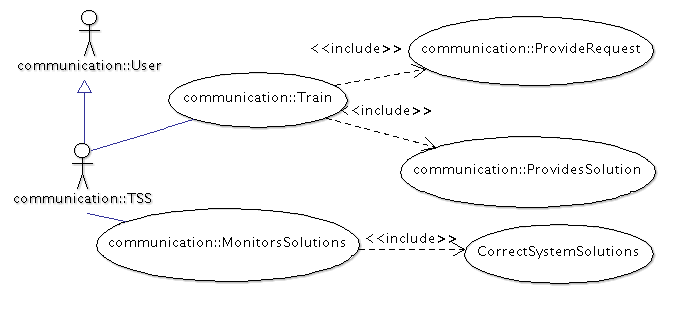
\includegraphics [scale=0.75] {UseCaseTrain}
  \caption{Вариант использования. Обучение} 
  \label{img:train}  
\end{figure}
Второй вариант использования~--- это основной поток. Главными действующим лицом системы является Заказчик (здесь и далее~--- Customer) (в общем случае это базовый класс Пользователь (здесь и далее~--- User)). Вариант использования имеет несколько ветвей, представленных в таблице \ref{ProductionUseCase}. В данном варианте система функционирует в «боевом режиме», то есть ищет ответ на запросы пользователя. В этом режиме есть возможность обучения: если система сталкнется с проблемой, то она задаст вопрос пользователю.
\begin{table} [htbp]
  \centering
  \parbox{15cm}{\caption{Описание ветвей в варианте использования «Основной режим»}\label{ProductionUseCase}}
%  \begin{center}
  \begin{tabular}{| p{10cm} | p{7cm} |}
 
  \hline
\textbf{Ветвь} & \textbf{Описание} \\
 
    \hline
ProvideRequest	& Заказчик вводит запрос в систему на естественном языке. Это могут быть либо прямая команда (например, Install Firefox, please), либо описание проблемы  \\
  \hline
communication:ProvideClarificationResponse  &  В случае, если система не может формализовать запрос либо нашлось множество решений, система запрашивает у пользователя детали
 \\
  \hline
communication:ProvideConfirmationResponse & В случае, когда система нашла решение, она запрашивает у пользователя подтверждение, что искомое решение решило его проблему
 \\

  \hline
  \end{tabular}
%  \end{center}
\end{table}
\clearpage
\subsection{Компоненты системы}
На рисунке \ref{img:MainComponentsCollaboration} представлено верхнеуровневое взаимодействие основных компонентов системы. В данном разделе будет дано краткое описание компонентов, последующие разделы будут посвящены отдельным компонентам, где будет представлено их подробное описание. В конце главы будет приведен подробный алгоритм взаимодействия всех компонентов системы.

\begin{figure} [h] 
  \center
  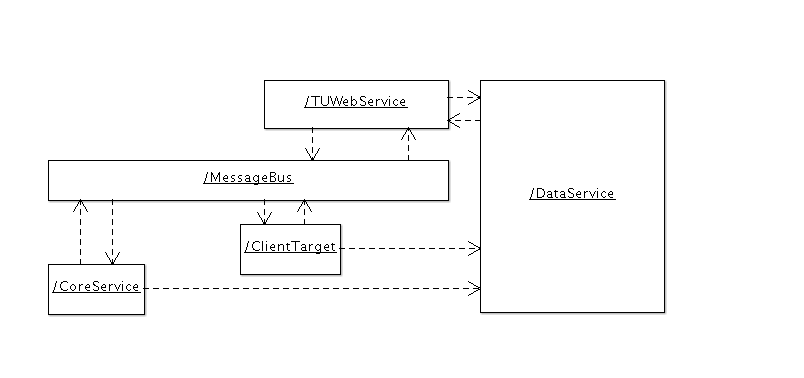
\includegraphics [scale=0.7] {MainComponentsCollaboration}
  \caption{Диаграмма взаимодействия компонентов} 
  \label{img:MainComponentsCollaboration}  
\end{figure}
Основной точкой взаимодействия (с позиции пользователя) с системой является компонент WebService (см. рисунок \ref{WebService}). Данный компонент построен на стандарте WS SOAP для универсального использования в различных внешних системах \cite{W1}. Взаимодействие происходит по следующей схеме:

\begin{enumerate}
	\item WebService получает запрос пользователя и сохраняет запрос в Базе Знаний (см. приложение \ref{Glossary});
	\item WebService отправляет сообщение типа Request с информацией о запросе в компонент MessageBus (шина);
	\item Один из экземпляров CoreService обрабатывает запрос;
	\item Компонент CoreService обрабатывает запрос и сохраняет результаты в Базе Знаний, затем он отправляет в MessageBus сообщение RequestCompleted и сообщение ActionsToExecute с указанием действий, которые необходимо исполнить;
	\item WebService получает сообщение RequestCompleted c результатами выполнения запроса и уведомляет подписчиков (конечных пользователей);
	\item Компонент ClientAgent получает сообщение ActionsToExecute со списком действий, которые необходимо исполнить на целевых машинах.
\end{enumerate} \par
Компонент MessageBus~--- это шина данных, которая обрабатывает сообщения и посылает их указанным компонентам. TUWebService~--- компонент взаимодействия с  «внешней средой», который предоставляет список функций и типов, посредством вызова которых можно обработать запрос в системе. Компонент DataService~--- отвечает за хранения данных, предоставляет базу заний для приложения. CoreService~--- ядро приложения, которое управляет основным жизненным циклом системы. ClientTarget~--- клиентский компонент для выполнения команд на машинах клиента. Сюда относятся как удаленное исполнение посредством WMI (Windows Management Instruments) и т.~п., так и непосредственная установка клиента на машины пользователей. На рисунке \ref{img:Component} (здесь и далее для детального изучения изображения, пожалуйста, воспользуйтесь функциями увеличения в pdf) представлено детальное описание компонентов с подкомпонентами. \par
Каждый верхнеуровневый компонент на рисунке \ref{img:Component} включает в себе более мелкие компоненты. Например, CoreService состоит из ThinkingLifeCycle~--- компонента управления жизненным циклом, Selector~--- компонента поиска и выбора ресурсов, Way2Think~--- компонента, описывающего алгоритмы поиска и применения решений и Critic~--- вероятностных триггеров, которые срабатывают на входящие события. Более детальное описание компонентов и механизмов представлено в остальных разделах данной главы. \par
В этой главе были представлены компоненты и их декомпозиция в разрезе системы. На рисунках видны крупноблочная структура системы, а также детальная~--- в разрезе общих блоков. Кроме того, описано взаимодействие с системой с точки зрения конечного пользователя, а также взаимодействия с другими системами. Также даны описание крупноблочных компонентов, а также детальное описание одного из основных компонентов.
\begin{figure} [h] 
  
  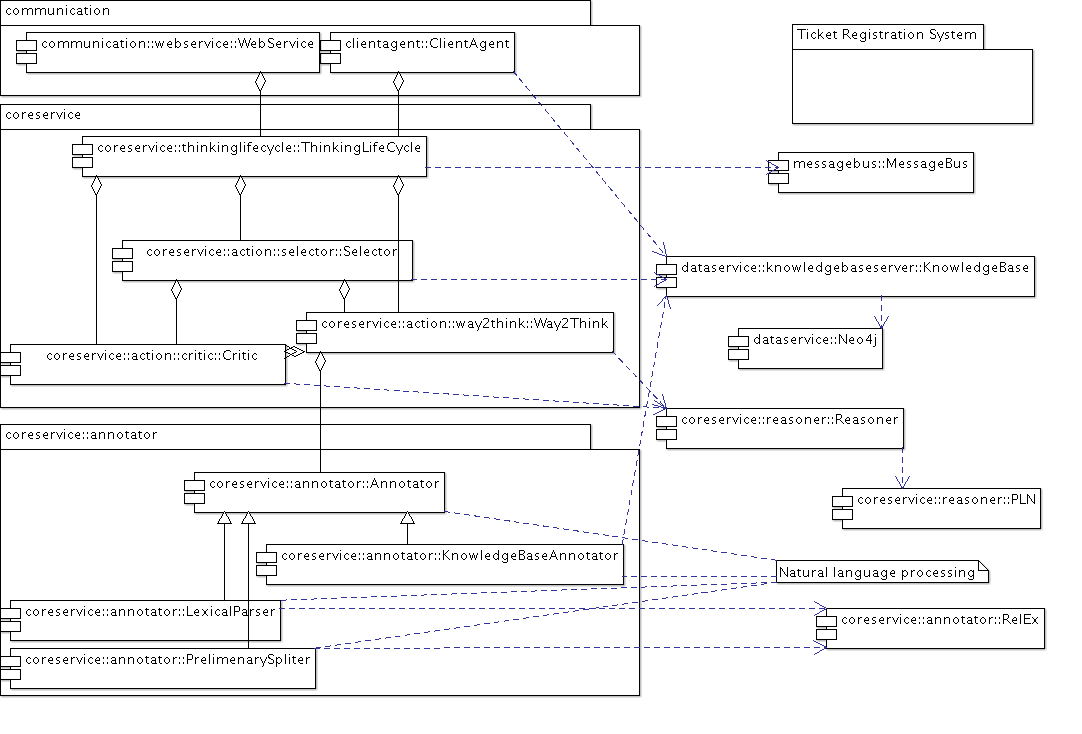
\includegraphics [scale=0.6, angle=90] {Component}
  \caption{Детальная диаграмма компонентов системы} 
  \label{img:Component}  
\end{figure}

\clearpage
\subsection{Компонент WebService} \label{WebService}
Данный компонент обрабатывает запросы пользователей, а также внешних систем. Запрос пользователя представляется посредством объекта Request, который содержит информацию о пользователя, а также ссылку на сервис пользователя, который будет вызван, когда запрос будет обработан. Вся работа происходит в компоненте CoreService.
На рисунке \ref{img:WebService} представлен интерфейс компонента.
В таблице \ref{WebServiceDescription} представлено описание методов.  
\begin{figure} [h] 
  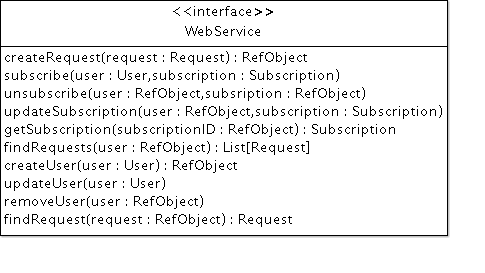
\includegraphics [width=0.8\textwidth,center] {WebService}
  \caption{Интерфейс компонента WebService} 
  \label{img:WebService}  
\end{figure}
Подробное описание классов представлено в приложении \ref{AppendixA}. Основной поток работы компонента состоит из следующих шагов:
\begin{enumerate}
	\item Пользователь создает запрос, используя метод WebService.createRequest;
	\item Система сохраняет запрос в Базе Знаний и начинает его обработку;
	\item Когда изменяется статус запроса (request.state), система оповещает подписчиков путем вызова ссылки на сервис пользователя, которая хранится в объекте Request.
\end{enumerate} \par
В общем виде данный компонент представляет фасад системы, ее внешнюю часть. Задача данного компонента~--- обеспечить легкое взаимодействие с системой и инкапсулировать основную логику системы. Соответствующие методы были подобраны так, чтобы внешним системам не нужно было реализовывать модель данной системы, а достаточно было использовать базовые облегченные объекты для приема и передачи информации. Данный подход подробно описан в книге Мартина Фаулера \cite{Patterns} и имеет название Data Transfer Object. В данном компоненте также широко используется подход Фасад, который также описан в названной книге. Архитектура компонента была проверена на предмет наличия антипаттернов проектирования, описанных в книге Вильяма Брауна \cite{AntiPatterns}. \par
В данном разделе был описан компонент взаимодействия с пользователям и внешними системами. Описаны архитектура компонента, основные методы, а также приведен пример основного потока.


\begin{table} [htbp]
   \center
   \parbox{15cm}{\caption{Описание методов компонента WebService}\label{WebServiceDescription}}
  \begin{tabular}{| p{8cm} |p{7cm} |}
  
  \hline
\textbf{Метод} & \textbf{Описание} \\
  \hline
  createRequest(request:Request): [RefObject] & Регистрирует запрос от пользователя. В качестве параметра в метод передается SubscriptionID, по которому идет проверка запроса \\
  
  \hline
  subscribe(user:User, subscription:Subscription)  & Создает подписку пользователя \\
  \hline
  unsubscribe(user:RefObject, subscription:RefObject)   & Убирает подписку пользователя \\
  \hline
  updateSubscription(user:RefObject, subscription:Subscription)   & Обновляет подписку пользователя \\
  \hline
  getSubscription(subscriptionID: RefObject): List<Request>    & Возвращает подписку \\
  \hline
  findRequests(user:RefObject)     & Возвращает запросы пользователя \\
  \hline
  createUser(user:User): RefObject     & Создает пользователя \\
  \hline
  updateUser(user:User)     & Обновляет информацию о пользователе \\ 
  \hline
  removeUser(user:RefObject)     & Удаляет информацию о пользователе \\ 
  \hline
  findRequest(request:RefObject): Request     & Возвращает запрос по ссылке \\ 
 
  \hline
\end{tabular}

\end{table}
\clearpage
\subsection{Компонент CoreService.ThinkingLifeCycle} \label{ThinkingLifeCycle}
Данный компонент системы отвечает за управление жизненным циклом системы: потоками, событиями приложения. Он запускает исполнение Критиков (Critic), Селекторов (Selector), Образов мышления (WayToThink), осуществляет обмен данных между компонентами. Компонент построен на фреймворке Akka Concurrency, который позволяет разрабатывать приложения, работающие параллельно \cite{AkkaConcurrency}. Архитектура модуля построена с учетом модели TU. \par
В данном компоненте реализовано шесть уровней мышления: Instinctive~--- инстинктивный уровень; Learned~--- уровень обученных реакций; Seliberative~--- уровень рассуждений; Reflective~--- рефлексивный уровень; Self-Reflective Thinking~--- саморефлексивный уровень; Self-Conscious Reflection~--- самосознательный уровень. \par

На уровне Instinctive идет обработка инцидентов, сгенерированных по шаблону.
Объект, который используется для обработки, применяет паттерн Akka \cite{AkkaConcurrency}. На рисунке \ref{img:ThinkingLifeCycle} представлена диаграмма классов компонента.  В таблице \ref{TLCCD} представлено подробное описание методов компонента с иллюстрациями. \par
На уровне Learned работают Критики классификации проблемы, они анализируют тип инцидента и активируют необходимые ресурсы. Более подробное описание работы Критиков приведено в следующих разделах. \par
На уровне Deliverative работает постановщик целей (который также является Критиком), который задает основные цели системы, тем самым запуская работу. Например, главная цель системы~--- решить проблему пользователя. Она активирует подцели, которые способствуют достижению основной цели. \par
На уровне Reflective работает Критик контроля времени, который отслеживает время выполнения запроса пользователя. \par
На уровне Self-Reflective Thinking осуществляется коммуникация с пользователем для уточнения запросов, проверки и применения найденного решения. \par
На уровне Self-Conscious работает Критик эмоционального состояния системы, который контролирует общее состояние системы и ее ресурсы. Критик контроля времени также обращается к этому критику для запроса ресурсов. \par
Данное расположение компонентов не случайно, оно реализует модель TU в привязке к различным уровням мышления. Проводя аналогию, можно сказать, что на более низких уровнях идет решение простых тактических задач, а на более высоких выстраивается общая стратегия поведения системы.
 
\begin{figure} [h] 
  \center
  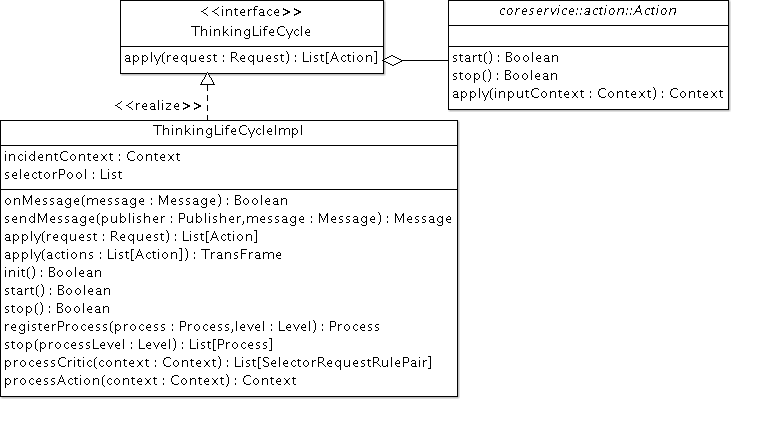
\includegraphics [scale=0.9,angle=90] {ThinkingLifeCycle}
  \caption{Диаграмма классов ThinkingLifeCycle} 
  \label{img:ThinkingLifeCycle}  
\end{figure}

\begin{longtable}{|p{7cm}|p{10cm}|}
 \caption[Описание методов класса (компонента) ThinkingLifeCycle]{Описание методов класса (компонента) ThinkingLifeCycle}\label{TLCCD} \\ 
 \hline
 
 \multicolumn{1}{|c|}{\textbf{Метод}} & \multicolumn{1}{c|}{\textbf{Описание}}  \\
\endfirsthead
\multicolumn{2}{c}%
{{\bfseries \tablename\ \thetable{} -- продолжение}} \\
\hline \multicolumn{1}{|c|}{\textbf{Метод}} &
\multicolumn{1}{c|}{\textbf{Описание}}  \\ \hline 
\endhead

\endfoot

\hline \hline
\endlastfoot
\hline
   onMessage(message : Message) & Данный метод вызывается при получении сообщения от шины. После этого происходит обработка запроса, формируется список действий, которые нужно выполнить. После этого запускается исполнение этих действий. На рисунке \ref{img:thinking-life-cycle-on-message-ad} представлена диаграмма действий этого метода \\
   \hline
   apply(request : Request) : List[Action] & Данный метод используется для запуска обработки входящего запроса. Для запроса создается контекст, если такой уже не был создан. После этого вызывается следующий компонент системы Selector, который выбирает необходимые ресурсы из Базы Знаний. На рисунке \ref{img:thinkinglifecycleapplyrequestRequestListAction} представлена диаграмма действий этого метода\\
   \hline
   apply(actions : List[Action]) : TransFrame & Данный метод запускает обработку действий. Все действия разделяются на Critic (триггеры действий, которые в итоге должны перейти в WayToThink через Selector) и WayToThink (образа мышления, непосредственые обработчики данных, классы, которые производят изменения данных). На рисунке \ref{img:thinkinglifecycleapplyactionsListActionTransFrame} представлена диаграмма действий этого метода \\
   \hline
   processWay2Think(inputContext: Context, outputContext: Context): TransFrame & Данный метод запускает обработку WayToThink. Он создает входной контекст (InputContext), заполняет его параметрами, создает выходной контекст OutputContext. Затем он запускает обработку данных во входном контексте. На рисунке \ref{img:thinkinglifecycleprocessWay2ThinkcontextContext} представлена диаграмма действий этого метода \\
    \hline
   processCritic(context: Context): List[SelectorRequestRulePair] & Данный метод запускает обработку Critic. На рисунке \ref{img:thinkinglifecycleactivityprocessCriticcontextContext} представлена диаграмма действий этого метода \\
   \hline
   init(): Boolean & Данный метод инициализирует экземпляр класса ThinkingLifeCycle. Во время инициализации происходят создание или подключение Базы Знаний (см. Словарь терминов \ref{Glossary}). На рисунке \ref{img:thinkinglifecycleinitBoolean} представлена диаграмма действий этого метода \\
    \hline
   start(): Boolean & Данный метод является необходимым для поддержки технологии Akka Concurrency, фактически он вызывает метод init \\
   \hline
   stop(): Boolean & Данный метод является необходимым для поддержки технологии Akka Concurrency, фактически он останавливает работу экземпляра класса: останавливается сессия к шине данных, останавливается подключение к Базе Знаний  \\
   \hline
   registerProcess(process : Process, level : Level) : Process & Данный метод ставит задачу в очередь исполнения. В качестве параметра принимается Level (уровень приоритета процесса) \\
   \hline
   stop(processLevel : Level) : List[Process] & Данный метод останавливает процесс. В качестве параметра принимается ссылка на процесс. На рисунке \ref{img:thinkinglifecyclestopprocessLevelLevelListProcess} представлена диаграмма действий этого метода  \\

 
 \hline 
\end{longtable}

\begin{figure} [h] 
  \center
  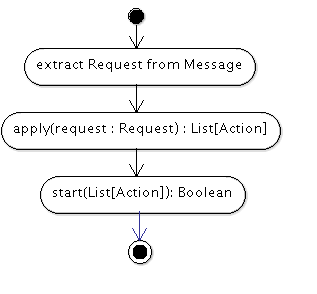
\includegraphics [scale=0.8] {thinkingLifeCycleonMessagemessageMessageBoolean}
  \caption{Диаграмма действий метода onMessage компонента ThinkingLifeCycle} 
  \label{img:thinking-life-cycle-on-message-ad}  
\end{figure}


\begin{figure} [h] 
  \center
  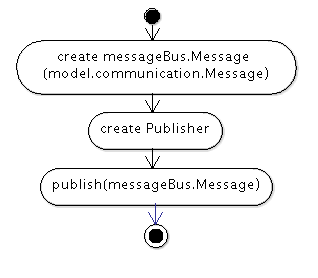
\includegraphics [scale=0.8] {thinkingLifeCyclesendMessagepublisherPublishermessageMessageMessage}
  \caption{Диаграмма действий метода sendMessage компонента ThinkingLifeCycle} 
  \label{img:thinking-life-cycle-send-message-publisher-publisher-ad}  
\end{figure}


\begin{figure} [h] 
  \center
  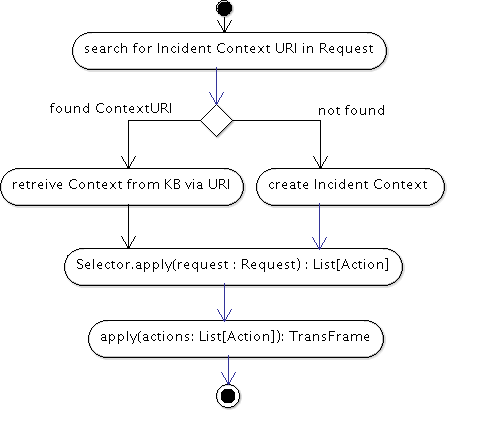
\includegraphics [scale=0.7] {thinkinglifecycleapplyrequestRequestListAction}
  \caption{Диаграмма действий метода apply компонента ThinkingLifeCycle} 
  \label{img:thinkinglifecycleapplyrequestRequestListAction}  
\end{figure}


\begin{figure} [h] 
  \center
  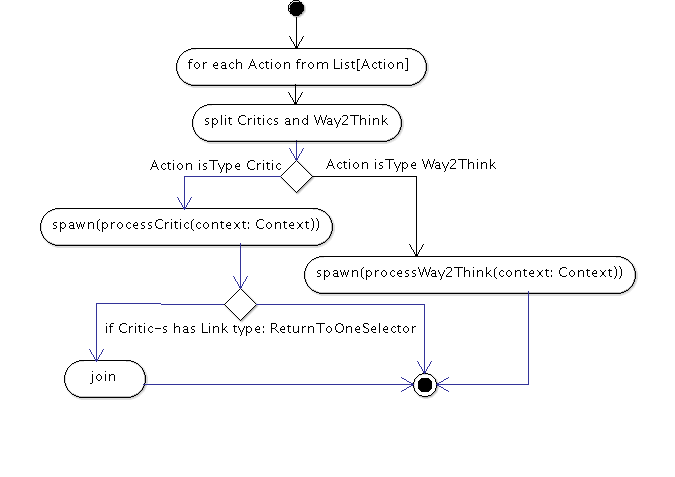
\includegraphics [scale=0.7] {thinkinglifecycleapplyactionsListActionTransFrame}
  \caption{Диаграмма действий метода apply компонента ThinkingLifeCycle} 
  \label{img:thinkinglifecycleapplyactionsListActionTransFrame}  
\end{figure}


\begin{figure} [h] 
  \center
  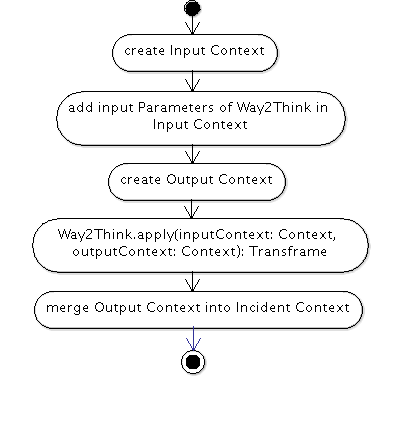
\includegraphics [scale=1.0] {thinkinglifecycleprocessWay2ThinkcontextContext}
  \caption{Диаграмма действий метода processWay2Think компонента ThinkingLifeCycle} 
  \label{img:thinkinglifecycleprocessWay2ThinkcontextContext}  
\end{figure}


\begin{figure} [h] 
  \center
  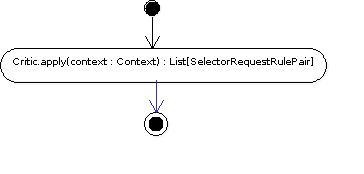
\includegraphics [scale=1.0] {thinkinglifecycleactivityprocessCriticcontextContext}
  \caption{Диаграмма действий метода processCritic компонента ThinkingLifeCycle} 
  \label{img:thinkinglifecycleactivityprocessCriticcontextContext}  
\end{figure}


\begin{figure} [h] 
  \center
  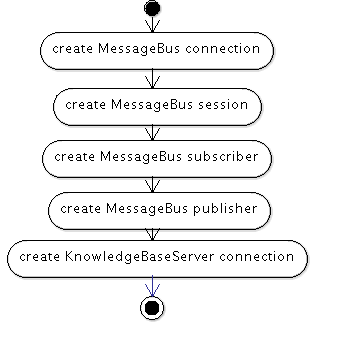
\includegraphics [scale=0.8] {thinkinglifecycleinitBoolean}
  \caption{Диаграмма действий метода init компонента ThinkingLifeCycle} 
  \label{img:thinkinglifecycleinitBoolean}  
\end{figure}

\begin{figure} [h] 
  \center
  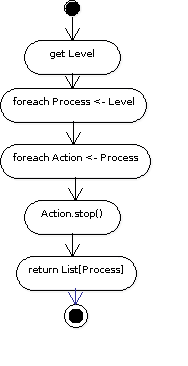
\includegraphics [scale=0.8] {thinkinglifecyclestopprocessLevelLevelListProcess}
  \caption{Диаграмма действий метода stop компонента ThinkingLifeCycle} 
  \label{img:thinkinglifecyclestopprocessLevelLevelListProcess}  
\end{figure}
\clearpage
\textbf{Описание работы компонента}. Чтобы понять работу компонента, далее рассмотрим описание алгоритма его работы. \par
\emph{Запуск и остановка}. Когда приложение запускается, оно инициализирует компонент ThinkingLifeCycle (далее TLC), который активирует набор критиков, базируясь на текущей цели системы. Например, если цель~--- классифицировать инцидент, то активируется набор критиков: разобрать, проверить, классифицировать. Когда приложение останавливается, оно останавливает все объекты класса и подклассов Actions (Critics, WayToThink), Selectors и ThinkingLifeCycle. \par
Коммуникация c остальными компонентами системы происходит посредством сообщений, отправленных через MessageBus (Шину Данных) JMS \cite{JMS}. Далее рассмотрим подробнее взаимодействие с остальными компонентами системы. \par
\begin{enumerate}
	\item Критик возвращает компоненту ThinkingLifeCycle (далее TLC) список Селекторов (SelectorRequestRule);
	\begin{enumerate}
	\item TLC запускает обработку компонента Selector;
	\item Selector возвращает TLC список Action (см. приложение \ref{AppendixB}) из Базы Знаний;
	\item TLC параллельно запускает возвращенные Action.
	\begin{enumerate}
	\item Если Action~--- это Critic;
	\item TLC создает InputContext (входной контекст приложения) и копирует туда все данные из Context (контекста) инцидента, созданного пользователем;
	\item Если Action~--- это Critic с ссылками ReturnToSameSelector, то TLC ждет результаты и отправляет компоненту Selector список SelectorRequestRule, которые были возвращены в качестве результата работы Critic. Иными словами, Critic может вернуть новый Selector. В данном случае нам нужно провести операцию Join для всех потоков \cite{JavaConcurrency}. В иных же случаях все Action запускаются в параллельных потоках.
	\end{enumerate} 
	\begin{enumerate}
	\item Если Action~--- это WayToThink;
	\item TLC создает InputContext (входной контекст приложения) и копирует туда все данные из Context (контекста), возвращенного Selector;
	\item TLC (см. таблицу \ref{Glossary}) запускает WayToThink;
	\item TLC сохраняет параметры в OutputContext;
	\item TLC сохраняет итоговый результат работы и возвращает его. 
	\end{enumerate} 
	\end{enumerate}
\end{enumerate} \par
В данном разделе было приведено описание основного цикла приложения с примерами работы. В следующих разделах содержится подробное описание работы каждого компонента на более низком уровне. В конце главы приведены развернутое описание стандартного цикла приложения и диаграмма расположения компонентов в разрезе уровней мышления.

%==============================
%==========Selector============
%==============================
\subsection{Компоненты \tripletshort} \label{Selector}\label{Critic}\label{WayToThink}
\textbf{Селектор (Selector)}~--- это компонент, который ответственен за получение списка действий и ресурсов из базы знаний, согласно входным параметрам. \par
\textbf{Входной критерий}. TLC запускает Selector c параметрами в виде контекста инцидента, который создал пользователь.  \par
\textbf{Выходной критерий}. Selector получает список Action: WayToThink или Critic. \par
\begin{figure} [h] 
  \center
  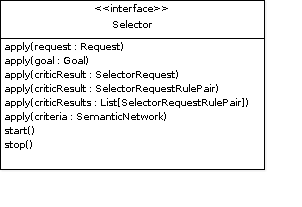
\includegraphics [scale=1.0] {SelectorInterface}
  \caption{Интерфейс компонента Selector} 
  \label{img:SelectorInterface}  
\end{figure} \par
На рисунке \ref{img:SelectorInterface} показан интерфейс компонент. В таблице \ref{SelectorMethodsDescription} приведено описание методов компонента.\\
\begin{longtable}{|p{7cm}|p{8cm}|}
 \caption[Описание методов класса (компонента) Selector]{Описание методов класса (компонента) Selector}\label{SelectorMethodsDescription} \\ 
 \hline
 
 \multicolumn{1}{|c|}{\textbf{Метод}} & \multicolumn{1}{c|}{\textbf{Описание}}  \\ \hline 
\endfirsthead
\multicolumn{2}{c}%
{{\bfseries \tablename\ \thetable{} -- продолжение}} \\
\hline \multicolumn{1}{|c|}{\textbf{Метод}} &
\multicolumn{1}{c|}{\textbf{Описание}}  \\ \hline 
\endhead

\endfoot

\hline \hline
\endlastfoot
\hline
  apply(request : Request) : Action & Данный метод на основе запроса пользователя получает из Базы знаний необходимые Critic \ref{Critic}. На рисунке \ref{img:applyrequestRequestActionActivity} представлена диаграмма действий этого метода \\
   \hline
   apply(goal: Goal) : Action & Данный метод на основе цели системы получает из Базы знаний необходимые Critic \ref{Critic}. На рисунке \ref{img:applygoalGoalActionActivity} представлена диаграмма действий этого метода\\
   \hline
   apply(criticResult : ActionProbabilityRule) : Action & Данный метод на основе работы Critic получает из Базы знаний необходимые Action. На рисунке \ref{img:applycriticResultActionProbabilityRulePairActionActivity} представлена диаграмма действий этого метода \\
 \hline 
\end{longtable}



\begin{figure} [h] 
  \center
  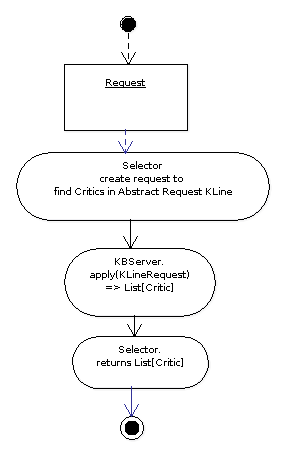
\includegraphics [scale=1.0] {applyrequestRequestActionActivity}
  \caption{Диаграмма действий метода Selector.apply(request : Request) компонента Selector} 
  \label{img:applyrequestRequestActionActivity}  
\end{figure}


\begin{figure} [h] 
  \center
  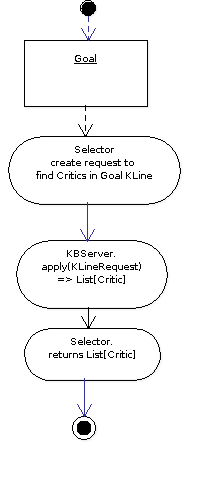
\includegraphics [scale=1.0] {applygoalGoalActionActivity}
  \caption{Диаграмма действий метода Selector.apply(goal: Goal) компонента Selector} 
  \label{img:applygoalGoalActionActivity}  
\end{figure}

\begin{figure} [h] 
  \center
  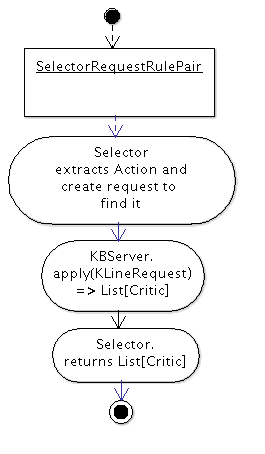
\includegraphics [scale=1.0] {applycriticResultActionProbabilityRulePairActionActivity}
  \caption{Диаграмма действий метода Selector.apply(criticResult : ActionProbabilityRule) компонента Selector} 
  \label{img:applycriticResultActionProbabilityRulePairActionActivity}  
\end{figure} \par



Чтобы лучше понять работу компонента и его назначение, далее рассмотрим сценарии его использования и взаимодействия с остальными компонентами на примере работы в режиме классификации входящего запроса.\par

\textbf{Действия при классификации входящего запроса} \par
\begin{enumerate}
	\item TLC (см. секцию \ref{ThinkingLifeCycle}) запускает входящие Critic (см. секцию \ref{Critic}) параллельно; 
	\item Когда Critic возвращает результат работы в виде ActionProbabilityRuleTriple, TLC запускает Selector с этим параметром;
	\item Selector запускает GetMostProbableWay2Think, который возвращает наиболее вероятный WayToThink;
	\item В некоторых случаях Selector может вернуть менее вероятный вариант, если на уровне мышления Reflective после проверки решения, оно было признано некорректным, или же пользователь признал его таким.
\end{enumerate} \par
На рисунке \ref{img:classifyIncidentActivity} представлена диаграмма действий классификации инцидента. TLC (см. секцию \ref{ThinkingLifeCycle}) получает цель классифицировать инцидент, затем Selector по этой цели возвращает Critic. После чего TLC запускает обработку Critic в разных потоках (параллельно). В данном случае рассматривается три Critic: DirectInstruction~--- прямые инструкции, данный Critic возвращает WayToThink Simulate (см. секцию \ref{WayToThink}), который ищет связь между концепциями в запросе и концепциями в Базе Знаний; ProblemWithDesiredState~--- проблема с ожидаемым результатом, данный Critic возвращает Simulate и Reformulate WayToThink, которые ищут сопоставление концепциями в Базе Знаний и пытается преобразовать запрос к DirectInstruction запросу (прямым инструкциям); ProblemWithoutDesiredState~--- проблема без ожидаемого результата, данный Critic возвращает Simulate, Reformulate, InferDesiredState, который пытается преобразовать проблему к ProblemWithDesiredState. \par
После работы компонента TLC (см. секцию \ref{ThinkingLifeCycle}) собирает результаты выполнения всех Critic и запускает их, пока не будет достигнута изначальная цель. \par
\begin{figure} [h] 
  \center
  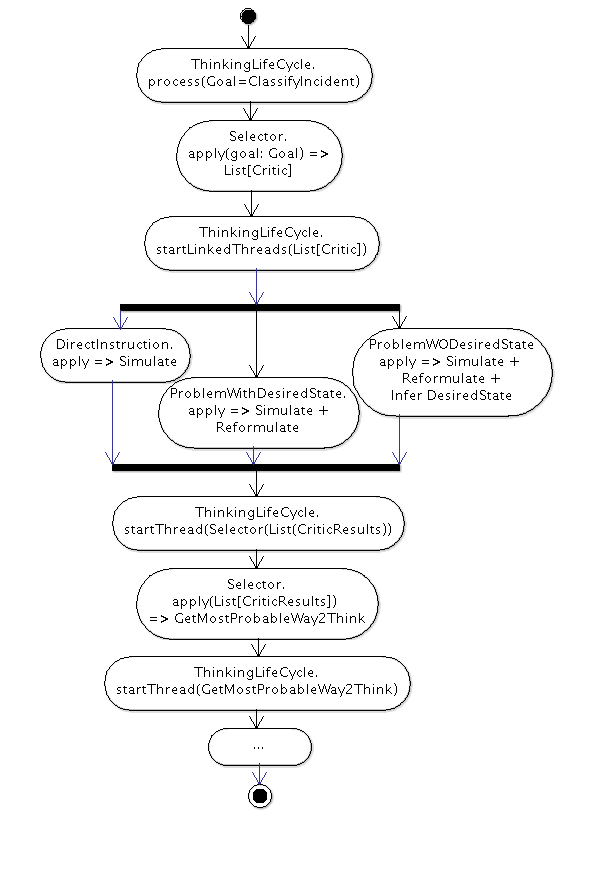
\includegraphics [scale=0.8] {classifyIncidentActivity}
  \caption{Диаграмма действий классификации инцидента} 
  \label{img:classifyIncidentActivity}  
\end{figure}
В данном разделе была описана работа компонента Selector с примерами работы и демонстрацией интеграции с остальными компонентами. Данный компонент тесно связан с компонентом TLC \ref{ThinkingLifeCycle}. Особенностью работы компонента является то, что список ресурсов, который он возвращает, можно задавать динамически, он также может формироваться во время работы системы. \par
\clearpage
%============================================
%===============Critic=======================
%============================================
\textbf{Critic} является основным компонентом для анализа в \tripletshort. Critic используется для классификации входной информации, рефлексии, само-анализа и служит определенным вероятностным переключатетелем. Например, компоненты контроля времени, контроля эмоционального состояния системы~--- это тоже Critic. \par
\textbf{Входной критерий}. TLC \ref{ThinkingLifeCycle} запускает Critic согласно Goal (Цель) (см. Приложение \ref{AppendixB}) или входящему запросу от пользователя. \par
\textbf{Выходной критерий}. Critic генерирует SelectorRequest \ref{Selector}. 
На входе Critic принимает: загруженные из базы правила для работы Critic (CriticRules); DomainModel:SemanticNetwork (см. \ref{acronyms})~--- доменная модель, представляющая собой семантическую сеть; описание инцидента, представляющее собой семантическую сеть. \par
На выходе Critic предоставляет: SelectorRequest \ref{Selector}~--- запрос на выбор Selector из базы знаний; CriticRule~--- правило, которое сработало для активации. Данное правило является логическим предикатом, т.~е. содержит в себе определенную формулу для вычисления вероятности. \par
На рисунке \ref{img:CriticApply} представлена диаграмма действий Critic, описание диаграммы приведено в таблице \ref{CriticMethods}.  В системе существуют разные типы Critic, их описание доступно в таблице \ref{CriticTypesRaw}.
\begin{figure} [h] 
  \center
  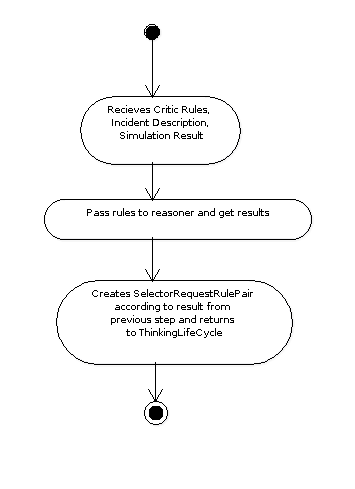
\includegraphics [scale=1.0] {CriticApply}
  \caption{Диаграмма действий компонента Critic} 
  \label{img:CriticApply}  
\end{figure}

\begin{longtable}{|p{7cm}|p{10cm}|}
 \caption[Описание основных типов Critic, используемых в системе]{Описание основных типов Critic, используемых в системе}\label{CriticTypesRaw} \\ 
 \hline
 
 \multicolumn{1}{|c|}{\textbf{Critic}} & \multicolumn{1}{c|}{\textbf{Описание}}  \\ \hline 
\endfirsthead
\multicolumn{2}{c}%
{{\bfseries \tablename\ \thetable{} -- продолжение}} \\
\hline \multicolumn{1}{|c|}{\textbf{Critic}} &
\multicolumn{1}{c|}{\textbf{Описание}}  \\ \hline 
\endhead

\endfoot

\hline \hline
\endlastfoot
\hline
   Manager & простой тип критика, который работает как триггер, например, Goal (см. приложение \ref{AppendixB}), который запускает необходимый WayToThink \\
   \hline
   Control & контролирующий Critic, который ждет определенного события (срабатывает на определенное событие). Например, заканчивается отведенное на решение время\\
   \hline
   Analyser & анализатор, обрабатывает и выявляет тип инцидента. Например, прямые инструкции, проблема с желаемым состоянием, выбор наиболее вероятного действия \\
 \hline 
\end{longtable}

\begin{longtable}{|p{8cm}|p{9cm}|}
 \caption[Описание методов компонента Critic]{Описание методов компонента Critic}\label{CriticMethods} \\ 
 \hline
 
 \multicolumn{1}{|c|}{\textbf{Метод}} & \multicolumn{1}{c|}{\textbf{Описание}}  \\ \hline 
\endfirsthead
\multicolumn{2}{c}%
{{\bfseries \tablename\ \thetable{} -- продолжение}} \\
\hline \multicolumn{1}{|c|}{\textbf{Метод}} &
\multicolumn{1}{c|}{\textbf{Описание}}  \\ \hline 
\endhead

\endfoot

\hline \hline
\endlastfoot
\hline
   exclude():List[CriticLink] & Данный метод возвращает список CriticLink, которые при срабатывание данного Critic будут игнорироваться с определенной вероятностью, после срабатывания Critic будет посчитана суммарная вероятность активации. После чего система решит, какой Critic был вероятнее всего активирован. \\
   \hline
   include():List[Critic] & Данный метод возвращает список объектов класса CriticLink, которые при срабатывание данного Critic будут включаться с определенной вероятностью.\\
   \hline
   apply(currentSituation: SemanticNetwork, domainModel:SemanticNetwork): List[SelectorRequestRulePair] & Данный метод запускает Critic, после чего вернется список Selector (см. секцию \ref{Selector}) с определенной веротяностью, после чего TLC (см. секцию \ref{ThinkingLifeCycle}) их активирует. \\
 \hline 
\end{longtable} 
Как сказано выше, Critic действуют на разных уровнях мышления. Далее приведено описание Critic с привязкой к уровням мышления.
\begin{enumerate}
	\item Уровень обученных реакций;
	\begin{enumerate}
		\item PreprocessManager~--- предобработка информации;
		\item Классификаторы инцидентов: Прямые инструкции, Проблема с желаемым состоянием, Проблема без желаемого состояния;
		\item SolutionCompletenessManager~--- связывается с пользователем и проверяет устраивает ли его найденное решение.
	\end{enumerate}
	\item Уровень рассуждений;
	\begin{enumerate}
		\item Выбор наиболее вероятного Selector по Rule. Данный Critic после проверки правил, выбирает из них правило с большей вероятностью.
	\end{enumerate}
	\item Рефлексивный уровень;
	\begin{enumerate}
		\item Менеджер целей. Установка целей.
	\end{enumerate}
	\item Саморефлексивный уровень;
	\begin{enumerate}
		\item ProcessingManager~--- запускает выполнение запроса;
		\item TimeControl~--- контроль времени исполнения запроса;
		\item DoNotUnderstandManager~--- активируется, когда необходимо уточнение пользователя для продолжения работы.
	\end{enumerate}
	\item Самосознательный уровень.
	\begin{enumerate}
		\item EmotionalStateManager~--- контроль общего состояния системы.
	\end{enumerate} 
\end{enumerate} \par
Основным примером работы компонента может служить классификация инцидентов (подробнее рассматривалось ранее). Например, у нас есть Critic для прямых инструкций DirectInstruction, есть для ситуации с желаемым состоянием DesiredState. Пусть на входе будет запрос вида: install antivirus. DesiredState найдет здесь действие~--- install, но не найдет желаемого состояния, то есть вероятность его выполнения будет 60\%. DirectInstruction будет искать действие и объект, которые присутствуют в запросе, его вероятность будет 100\%, его TLC (см. секцию \ref{ThinkingLifeCycle}) и активируют как наиболее вероятный. \par
Это был простой пример работы компонента, на самом деле механизм работы гораздо гибче: он поддерживает включения, исключения, составные правила и логику. Компонент также является динамически формируемым. \par
В данном разделе был описан важный компонент системы, который определяет алгоритм ее работы, в этом компоненте скрыта основная возможность системы думать и решать, согласно набором правил и внешним обстоятельствам. \par

%=================================
%===========WayToThink============
%=================================
\textbf{WayToThink} является основным операционным компонентом \tripletshort. Основными задачами данного компонента являются: обновление, преобразование, сохранение данных и коммуникация с пользователем, иными словами, все, что в той или иной форме изменяет операционный контекст данных системы. \par
\textbf{Входной критерий}. Запуск осуществляется из компонента ThinkingLufeCycle (см. секцию \ref{ThinkingLifeCycle}). Входными данными является InputContext, который содержит параметры WayToThink.\par
\textbf{Выходной критерий}. WayToThink завершил работу. На выходе возвращают измененные в ходе работы данные. В общем виде компонент описывает последовательность действий. В системе используется два больших класса WaytToThink~--- простой и составной (сложный). Простые WayToThink являются встроенными в систему, остальные являются комбинацией компонентов: Critic \ref{Critic}, Selector \ref{Selector}, WayToThink \ref{WayToThink}. В таблице \ref{WayToThinkList} приведено описание встроенных в систему WayToThink. На рисунке \ref{img:Way2ThinkInterface} представлен интерфейс компонента. В таблице \ref{WayToThinkMethods} представлено описание методов WayToThink.  

\begin{figure} [h] 
  \center
  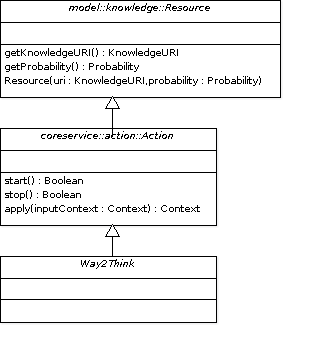
\includegraphics [scale=0.8] {Way2ThinkInterface}
  \caption{Интерфейс компонента WayToThink} 
  \label{img:Way2ThinkInterface}  
\end{figure}

\begin{longtable}{|p{7cm}|p{10cm}|}
 \caption[Описание встроенных в систему WayToThink]{Описание встроенных в систему WayToThink}\label{WayToThinkList} \\ 
 \hline
 
 \multicolumn{1}{|c|}{\textbf{WayToThink}} & \multicolumn{1}{c|}{\textbf{Описание}}  \\ \hline 
\endfirsthead
\multicolumn{2}{c}%
{{\bfseries \tablename\ \thetable{} -- продолжение}} \\
\hline \multicolumn{1}{|c|}{\textbf{WayToThink}} &
\multicolumn{1}{c|}{\textbf{Описание}}  \\ \hline 
\endhead

\endfoot

\hline \hline
\endlastfoot
\hline
   Создать контекст & Данный WayToThink создает объект Context для аккумуляции данных запроса \\
   \hline
   Установить общий статус системы & Данный WayToThink устанавливает состояние системы в глобальном контексте\\
   \hline
   Установить цель системы & Данный WayToThink устанавливает цель запроса в текущем контексте  \ref{AppendixB} \\
    \hline
   Разделить фразу на слова и предложения & Данный WayToThink разбивает фразу на слова и возвращает список слов\\
    \hline
   Найти связи между входной информацией и базой знаний & Данный WayToThink ищет связь между входной информацией и базой знаний\\ 
   \hline
   Извлечь связи & Данный WayToThink возвращает список связей из фразы\\
    \hline
   Сохранить наиболее вероятное решение & Данный WayToThink сохраняет наиболее вероятное решение\\
    \hline
   Перефразировать (Reformulate) & Данный WayToThink ищет связь между текущим контекстом и известными проблемами, если есть неизвестные концепции, то он пытается их переформулировать при помощи пользотеля\\
   \hline
   Смоделировать (Simulate) & Данный WayToThink ищет связь между текущим контекстом и проблемами уже сохраненными в базе\\
   \hline
   Найти решение & Данный WayToThink производит поиск решения, которое прикреплено к проблеме, которая была найдена при помощи моделирования и перефразирования\\
   \hline
   Остановить работу & Данный WayToThink останавливает работу системы\\
 \hline 
\end{longtable}

\begin{longtable}{|p{7cm}|p{10cm}|}
 \caption[Описание методов компонента WayToThink]{Описание методов компонента WayToThink}\label{WayToThinkMethods} \\ 
 \hline
 
 \multicolumn{1}{|c|}{\textbf{Метод}} & \multicolumn{1}{c|}{\textbf{Описание}}  \\ \hline 
\endfirsthead
\multicolumn{2}{c}%
{{\bfseries \tablename\ \thetable{} -- продолжение}} \\
\hline \multicolumn{1}{|c|}{\textbf{Метод}} &
\multicolumn{1}{c|}{\textbf{Описание}}  \\ \hline 
\endhead


\endfoot

\hline \hline
\endlastfoot
\hline
   start() & Запустить обработку информации \\
   \hline
   stop() & Остановить обработку, например, если выполнение идет слишком долго\\
   \hline
   apply(inputContext:Context): Context & Применить WayToThink. Исполнение начнется только после вызова метода start \\
    \hline
\end{longtable}

WayToThink также используется как описание алгоритма разрешения проблемы (см. приложение \ref{AppendixDHowTo} HowTo), то есть описывает последовательность действий, необходимых для устранения проблемной ситуации. \par
В зависимости от типа WayToThink активируется та или иная последовательность действий. В общем виде последовательность имеет следующий вид: получить данные, обработать, вернуть данные. В случае, например, WayToThink Simulate второй шаг имеет вид «найти связь между текущим контекстом и проблемами, уже сохраненными в Базе Знаний». Если же WayToThink является описанием решения, то второй шаг может быть набором вызова системных утилит с параметрами из первого шага. \par
В данном разделе был описан основной компонент модификации данных WayToThink. Нужно отметить, что данный компонент также является важной частью модели TU. Проектировался он для универсального применения во всех случаях, когда необходимо действие над данными. Например, если нужно использовать скрипт, который был написан на языке интерпретации Bash, и ввести его в систему, можно разбить каждый шаг и вызов на отдельную часть и сделать сложный WayToThink с ветвлениями и циклами. \par
\begin{figure} [h] 
  \center
  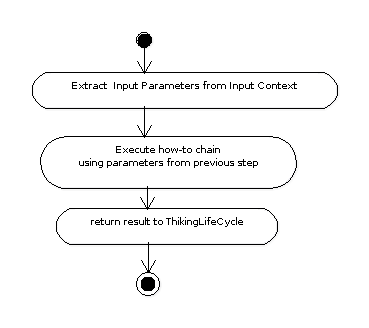
\includegraphics [scale=0.8] {way2thinkHowToActivity}
  \caption{Работа компонента WayToThink в режиме описания решения проблемы (HowTo) } 
  \label{img:way2thinkHowToActivity}  
\end{figure}
%===================================
%===========PreliminaryAnnotator====
%===================================
\clearpage
\subsection{Вспомогательные компоненты} \label{PreliminaryAnnotator}\label{KnowledgeBaseAnnotator}\label{data service}\label{Reasoner}
Данный компонент проводит предварительную подготовку текста: грамматическую и орфографическую коррекции текста, а также разделение на предложения. На рисунке \ref{img:PrelimenaryAnnotatorInterface} представлен интерфейс компонента. Компонент также является WayToThink, так как он производит модификацию данных контекста. В таблице \ref{PrelimenaryAnnotatorMethods} приведено описание методов класса.
\begin{figure} [h] 
  \center
  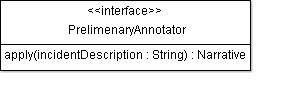
\includegraphics [scale=1.0] {PrelimenaryAnnotatorInterface}
  \caption{Интерфейс компонента PrelimenaryAnnotator} 
  \label{img:PrelimenaryAnnotatorInterface}  
\end{figure}
\begin{longtable}{|p{7cm}|p{10cm}|}
 \caption[Описание методов компонента PrelimenaryAnnotator]{Описание методов компонента PrelimenaryAnnotator}\label{PrelimenaryAnnotatorMethods} \\ 
 \hline
 
 \multicolumn{1}{|c|}{\textbf{Метод}} & \multicolumn{1}{c|}{\textbf{Описание}}  \\ \hline 
\endfirsthead
\multicolumn{2}{c}%
{{\bfseries \tablename\ \thetable{} -- продолжение}} \\
\hline \multicolumn{1}{|c|}{\textbf{Метод}} &
\multicolumn{1}{c|}{\textbf{Описание}}  \\ \hline 
\endhead


\endfoot

\hline \hline
\endlastfoot
\hline
   apply(incidentDescription:String): Narrative & Данный метод запускает обработку входного текста и его корректировку \\
   \hline
  \end{longtable}
С точки зрения корректировки текст подвергается обработке средствами проверки языка, например, открытый комплекс After the deadline \cite{AfterTheDeadline}, а также Google API. В части разбиения текста на слова используется алгоритм из открытого комплекса Link Grammar \cite{LG-2}. В целом компонент содержит в себе также составную системы разбора, что отличает его от прямого использования алгоритма. Он манипулирует результатом работы из нескольких подсистем, для увеличения степени точности. \par
Одной из особенностью компонента является использование внутренней базы знаний для предобработки текста, чтобы убрать неточности, которые будут мешать работе средств NLP. Например, часто средства NLP не понимают концепцию слова please, поэтому в базе изначально хранится эта концепция с правильным значением. Таким образом, на вход средствам NLP поступает уже аннотированный текст, что позволяет на 20\% (согласно экспериментальным данным) увеличить точность обработки. \par
%===================================
%===========KnowledgeBaseAnnotator==
%===================================
\textbf{Компонент CoreService.KnowledgeBaseAnnotator}\par 
Данный компонент устанавливает связи между терминами во входной фразе и базой знаний и также является WayToThink \ref{WayToThink}.  \par
\textbf{Входные критерии}. Список подготовленных фраз в виде объектов. \par
\textbf{Выходные критерии}. Список ссылок на внутренние знания. \par
\textbf{Описание работы компонента} \par
\begin{enumerate}
	\item Получен Термин;
	\item Поиск в локальной базе знаний;
	\item Если совпадение не найдено идет запрос во внешнюю базу знаний;
	\item Внешняя база возвращает список синонимов;
	\item Компонент ищет по синонимам во внутренний базе знаний;
	\item Если поиск успешен, то создается связь между входящем термином, синонимом и концепцией в базе знаний.
\end{enumerate}
Например, входящий запрос содержит термин "program"\,, база знаний содержит термин "computer software". Идет запрос во внешние базы знаний, найдено "computer software, program". Будет добавлена связь-аналогия в база знаний "program~--- computer software". 


%===================================
%===========DataService==
%===================================
\textbf{Компонент DataService} \par
Данный компонент отвечает за хранение данных в системе. База знаний построена на графах. На рисунке \ref{img:KnowledgeBaseServer} представлен интерфейс компонента. В базе знаний используется два типа объектов Object~--- объект базы знаний, BusiessObject~--- объект для Web Service (User, Request). BusinessObject является кортежем для интеграции с внешними системами. У объекта есть ID, который уникально удостоверяет его в рамках системы. В таблице \ref{DataServiceMethods} приведено описание методов компонента. \par
\begin{figure} [h] 
  \center
  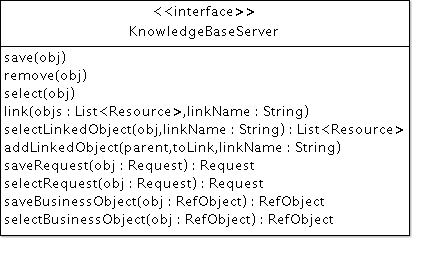
\includegraphics [scale=0.8] {KnowledgeBaseServer}
  \caption{Интерфейс компонента KnowledgeBaseServer} 
  \label{img:KnowledgeBaseServer}  
\end{figure}
\begin{longtable}{|p{8cm}|p{9cm}|}
 \caption[Описание методов компонента DataService]{Описание методов компонента DataService}\label{DataServiceMethods} \\ 
 \hline
 
 \multicolumn{1}{|c|}{\textbf{Метод}} & \multicolumn{1}{c|}{\textbf{Описание}}  \\ \hline 
\endfirsthead
\multicolumn{2}{c}%
{{\bfseries \tablename\ \thetable{} -- продолжение}} \\
\hline \multicolumn{1}{|c|}{\textbf{Метод}} &
\multicolumn{1}{c|}{\textbf{Описание}}  \\ \hline 
\endhead


\endfoot

\hline \hline
\endlastfoot
\hline
   save(obj:Resource): Resource  & Данный метод позволяет сохранить ресурс в базу знаний \\
   \hline
   remove(obj:Resource)  & Данный метод позволяет удалить объект \\
   \hline
   select(obj:Resource): Resource  & Данный метод позволяет выбрать объект \\
   \hline
   link(obj:List<Resource>, linkName:String)  & Данный метод позволяет сделать ссылку между 2-мя объектами \\
   \hline
   selectLinkedObject(obj:Resource, linkName:String): Link<Resource>  & Данный метод позволяет выбрать все объекты, которые имеют связь под названием linkName с объектом obj \\
   \hline
   addLinkedObject(parent:Resource, toLink:Resource, linkName:String)  & Данный метод позволяет создать ссылку linkName с объектом \\
   \hline
   saveRequest(obj:Request)  & Данный метод позволяет получить запрос из Базы Знаний \\
   \hline
   selectRequest(obj:RefObject)  & Данный метод позволяет получить запрос из Базы Знаний \\
   \hline
   saveBusinessObject(obj:RefObject): RefObject  & Данный метод позволяет сохранить объект в базу \\
   \hline
   selectBusinessObject(obj:RefObject): RefObject  & Данный метод позволяет полуить объект из Базы Знаний \\
   \hline
  \end{longtable}

%=================================
%===========Reasoner===========
%=================================
\textbf{Компонент Reasoner} \par
Данный компонент осуществляет логические вычисления для системы, например, для обработки правил в компоненте Critic \ref{Critic}. На рисунке \ref{img:ReasonerInterface} представлен интерфейс компонента. В таблице \ref{ReasonerMethods} приведено описание методов компонента. 
%ReasonerInterface.png 
\begin{figure} [h] 
  \center
  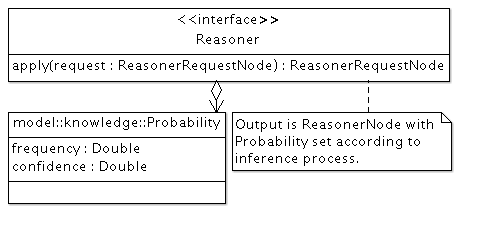
\includegraphics [scale=0.8] {ReasonerInterface}
  \caption{Интерфейс компонента Reasoner} 
  \label{img:ReasonerInterface}  
\end{figure}
\begin{longtable}{|p{7cm}|p{10cm}|}
 \caption[Описание методов компонента Reasoner]{Описание методов компонента Reasoner}\label{ReasonerMethods} \\ 
 \hline
 
 \multicolumn{1}{|c|}{\textbf{Метод}} & \multicolumn{1}{c|}{\textbf{Описание}}  \\ \hline 
\endfirsthead
\multicolumn{2}{c}%
{{\bfseries \tablename\ \thetable{} -- продолжение}} \\
\hline \multicolumn{1}{|c|}{\textbf{Метод}} &
\multicolumn{1}{c|}{\textbf{Описание}}  \\ \hline 
\endhead

\endfoot

\hline \hline
\endlastfoot
\hline
   apply(request: ReasonerRequestNode): ReasonerRequestNode  & Данный метод проводит обработку правил и считает вероятность (Probability) и уверенность (Confidence) \\
   \hline
  
  \end{longtable}
На данный момент в качестве реализации в системе используется два движка логический вычисление PLN \cite{PLN} и NARS \cite{NARS}. Основным применением данного компонента являются правила для Critic. Логика правил обрабатывается при помощи этого компонента. Этот результат используется для определения вероятности активации данного Critic. Подобное использование дает гибкость в построении свода правил. 
  
\clearpage
%=================================
%===========Knowledge=============
%=================================
\section{Модель данных TU Knowledge} 
Одной из важных частей системы является реализация хранения данных на основе модели TU. Для работы системы была разработана уникальная схема данных~--- TU Knowledge, которая сочетает в себе OWL и графовую базу данных. Язык OWL, традиционно использующийся для структурирования информации в Вебе \cite{OWL}, обрел широкое использование во многих схемах данных, так как давал возможность дополнительного расширенного описания взаимосвязи между данными. На рисунке \ref{img:KnowledgeClass} представлена схема данных TU Knowledge. В таблице \ref{TUKnowledge} представлено описание схемы TU Knowledge.
\begin{figure} [h] 
  \center
  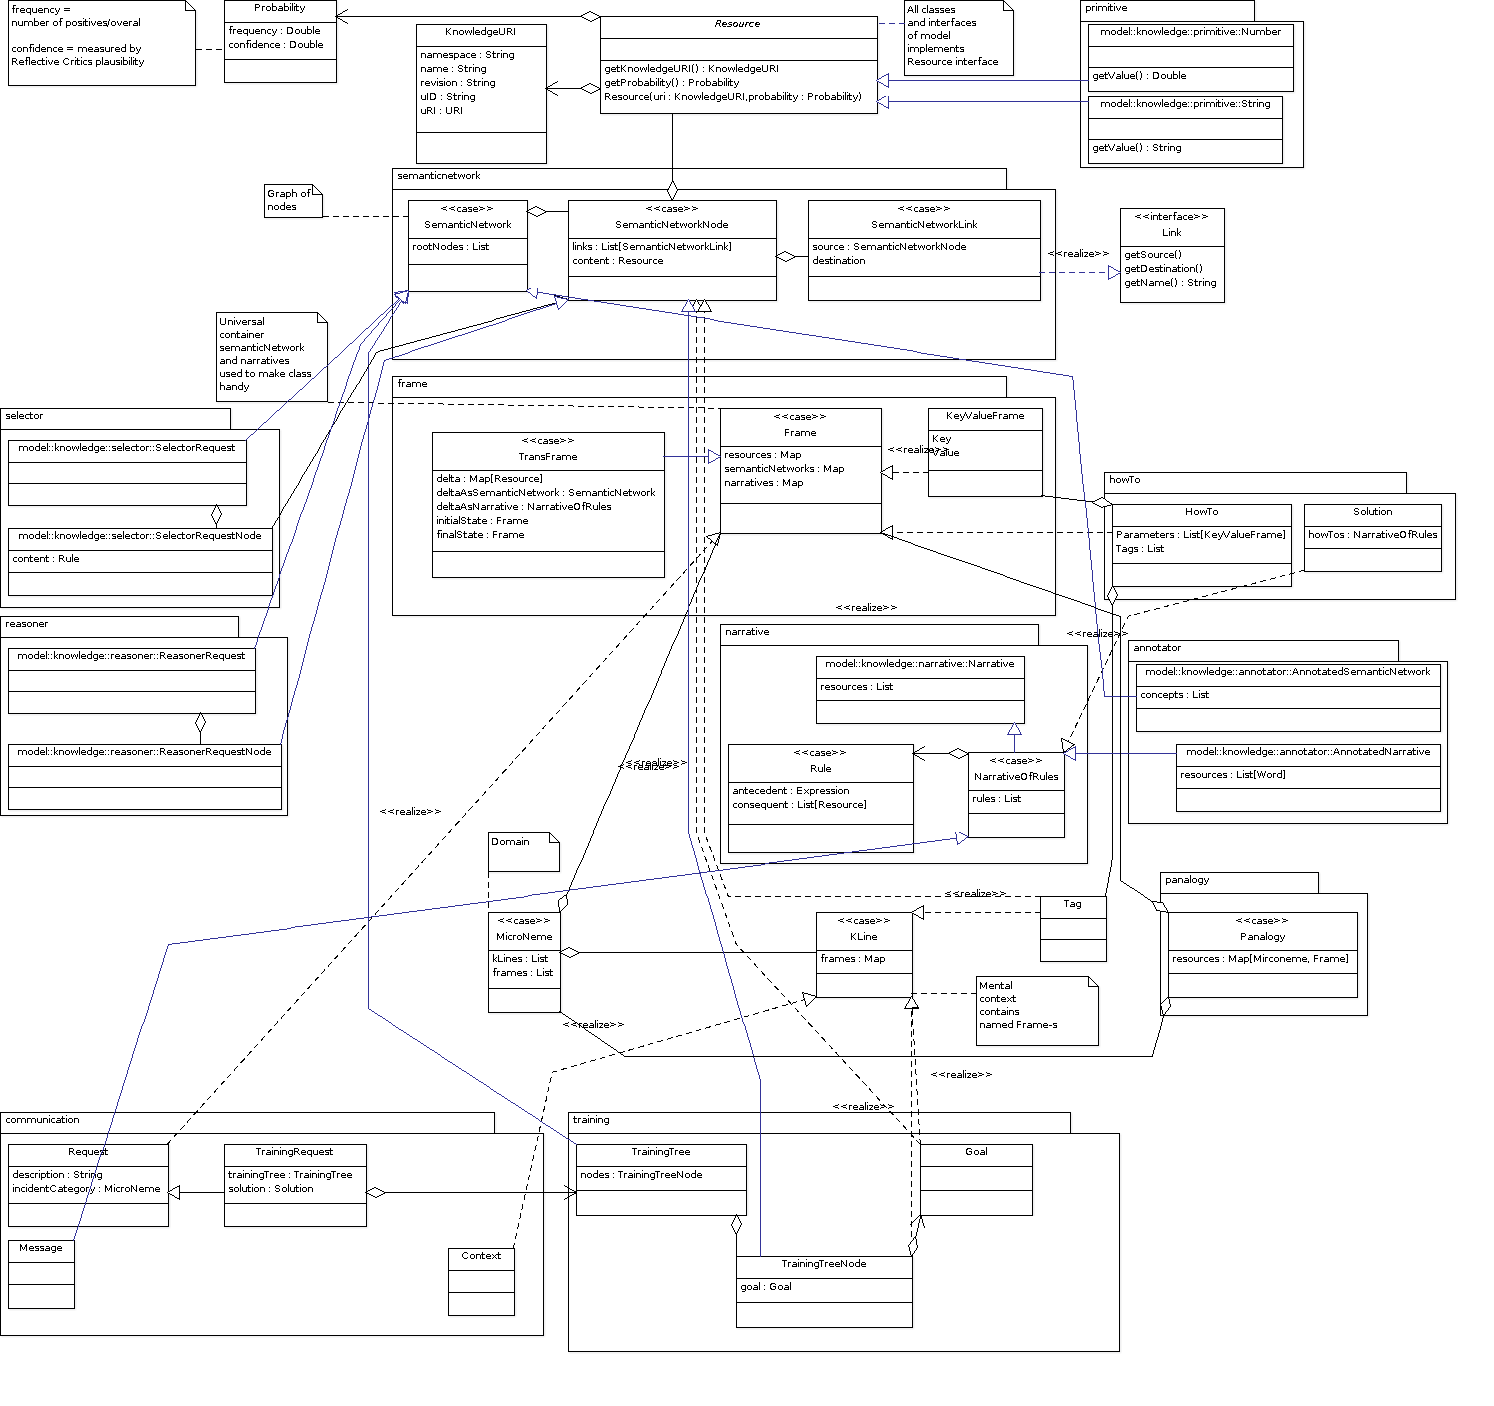
\includegraphics [scale=0.33] {KnowledgeClass}
  \caption{Схема данных TU Knowledge в формате UML} 
  \label{img:KnowledgeClass}  
\end{figure}

\begin{longtable}{|p{5cm}|p{12cm}|}
 \caption[Описание классов TUKnowledge]{Описание классов TUKnowledge}\label{TUKnowledge} \\ 
 \hline
 
 \multicolumn{1}{|c|}{\textbf{Класс}} & \multicolumn{1}{c|}{\textbf{Описание}}  \\ \hline 
\endfirsthead
\multicolumn{2}{c}%
{{\bfseries \tablename\ \thetable{} -- продолжение}} \\
\hline \multicolumn{1}{|c|}{\textbf{Класс}} &
\multicolumn{1}{c|}{\textbf{Описание}}  \\ \hline 
\endhead

\endfoot

\hline \hline
\endlastfoot
\hline
   Knowledge  & Базовый класс всех объектов модели. Содержит в себе URI, по которому уникально идентифицируется. Поддерживает версионность. Свойствами данного объекта обладают все объекты системы. Также содержит Probability (Вероятность) и Confidence (Уверенность) поля. Например, когда в результате работу WayToThink получается Knowledge он имеет Confidence 0, так как он только что был сгенерирован, когда его проверит Critic на его состоятельность при помощи определенных в Critic правил, то он поставит ему не 0 Confidence \\
   \hline
   Narrative  & Список слов исходного запроса \\
   \hline
   Rule  & Правило. Класс описывающий правила в системы. Например, правило по которому сработает Critic \ref{Critic}  \\
   \hline
   AnnotatedNarrative  & Слова исходного запроса и их сопоставление на концепции в Базе Знаний \\
   \hline
   SemanticNetwork  & Граф из SemanticNetworkNode и SemanticNetworkLink \\
   \hline
   SemanticNetworkNode  & Узел графа SemanticNetwork, содержит в себе ссылки на другие узлы, а также ссылку на Knowledge \\
   \hline
   SemanticNetworkLink  & Ссылка в графе SemanticNetworkLink \\
   \hline
   Frame  & Коллекция объектов Knowledge, с возможностью назначения специального атрибута (тега) для семантической группировки \\
   \hline
   TransFrame  & Коллекция Frame, содержащая два состояния одного фрейма: до и после \\
   \hline
   Goal  & Цель. Приложение \ref{AppendixB} \\
   \hline
   Tag & То же, что и цель, но используется для меток \\
   \hline
   Preliminary annotation  & SemanticNetwork входного запроса \\
   \hline
   KnowledgeBase annotation  & SemanticNetwork с сопоставлением концепциям Базы Знаний \\
   \hline
   Domain model  & SemanticNetwork доменной модели \\
   \hline
   Situation model  & SemanticNetwork, часть DomainModel, созданной для обработки текущего запроса. Приложение \ref{AppendixB} \\
   \hline
   Incident  & SemanticNetwork входного запроса к систему \\
   \hline
   K-Line  & Связь между объектами. Например, когда в систему поступает запрос она создает K-Line между Conversation, Narrative \\
   \hline
   Conversation  & SemanticNetwork, контекст инцидента \\
   \hline
   InboundRequest  & SemanticNetwork входного запроса \\
   \hline
   Training Request  & SemanticNetwork входного запроса для обучений \\
   \hline
   
  \end{longtable}

\textbf{Описание запросов в рамках TU Knowledge} \par
В рамках модели данных TU Knowledge проблема имеет следующее описание:
\begin{itemize}
	\item Область (Микронема);
	\item Дата обращения;
	\item Автор;
	\item Приоритет;
	\item Категория;
	\item Теги;
	\item Описание.
\end{itemize}
Запрос на обучение включает следующие части:
\begin{itemize}
	\item Область (Микронема);
	\item Дерево обучения;
	\item Ограничения (например, время на решение).
\end{itemize} \par
 \textbf{Микронема} описывает контекст работы системы. В разрезе человеческого мышления это область работы мозга с нейронами и связями. Сочетание разных микронем может привести к изменению взглядов человека, характера, например, когда кто-то узнает новую идею и это заменяет его предыдущие представления о том или ином явлении. \par 

\textbf{Дерево обучения} базируется на структуре цель--подцель (см. приложение \ref{AppendixB}). Получение системой целей происходит из подцелей или при получении запроса пользователя. Например, при запросе пользователя устанавливается цель "Help User (Помочь пользователю)".\par

Во время процедуры обучения возможно, что на одном уровне окажется несколько целей, тогда необходимо провести дополнительное уточнение, если такое невозможно, то будет выбрана первая цель.


Во время работы MostProbableWay2Think может использовать несколько WayToThink, в таком случае он возьмет первый (наиболее вероятный путь). Если в результате его использования цель достигнута не будет, то будет выбран менее вероятный.

Пример
\begin{lstlisting}
 1. SubGoal = Resolve incident
   2. SubGoal = ParseIncidentDescription, Way2Think = ProcessText: KnowingHow, SemanticNetWorkWithKLines =
{
nsubj(received-3, User-1)
aux(received-3, had-2)
root(ROOT-0, received-3)
amod(application-5, wrong-4)
dobj(received-3, application-5)

advmod(received-3, However-1)
nsubj(received-3, user-2)
ccomp(received-8, received-3)
amod(version-5, wrong-4)
dobj(received-3, version-5)
nsubj(received-8, user-7)
root(ROOT-0, received-8)
nn(Tehcnical-10, Wordfinder-9)
dobj(received-8, Tehcnical-10)
advmod(of-12, instead-11)
prep(Tehcnical-10, of-12)
nn(Economical-14, Business-13)
pobj(of-12, Economical-14)
}
   2. SubGoal = UnderstandIncidentType, Critics = Deliberative, Type = ProblemDescription with DesiredState
     3. SubGoal = ModelCurrentSituation using ProjectDomain Model, Way2Think = Simulate, Model =
{
User Desired(ordered) Soft(Wordfinder Business Economical)
Operator Installed Soft(Wordfinder Tehcnical) - wrongly
}
     3. SubGoal = FormalizeProblemDescription using ProblemModel(Wrong state, Desired state), Way2Think = Reformulate, Model=
{
WrongState = Soft.installed(Wordfinder Tehcnical), Soft.notInstalled(Wordfinder Business Economical)
DesiredState = Soft.installed(Wordfinder Business Economical), Soft.unInstalled(Wordfinder Tehcnical)
}
     3. SubGoal = Find solution, Way2Think = ExtendedSearch, Solution =
     { Install(Wordfinder Business Economical), UnInstall(Wordfinder Tehcnical)}
     
\end{lstlisting}
\clearpage

\section{Прототип системы}
В прототипе были реализованы 4 уровня мышления. Ниже описан стандартный поток системы, который дает возможность понять основной принцип работы.
\begin{enumerate}
	\item Поступает запрос пользователя: 
	"User had received wrong application. User has ordered Wordfinder Business Economical. However she received wrong version, she received Wordfinder Tehcnical instead of Business Economical. Please assist."\ («Пользователь получил неверное приложение. Пользователь заказал приложение "Wordfinder. Бизнес версия"\,, но получил неверную версию,~--- "Wordfinder. Техническая версия". Пожалуйста, помогите»);
	\item Компонент GoalManger (Менеджер целей) устанавливает цель системы HelpUser (Помочь пользователю);
	\item Главный компонент Thinking Life Cycle (далее TLC) активирует набор компонетов Critic (Критик), привязанный к данной цели (HelpUser); 
	\item Активируется компонент PreliminaryAnnorator (Предварительный обработчик), который разбирает запрос, проводя орфографическую коррекцию и предварительный разбор;
	\item Компонент KnowledgeBaseAnnotator (разбор при помощи накопленных знаний) создает семантическую сеть и ссылки на нее;
	\item Компонент Critic (Критик), привязанный к цели HelpUser на Рефлексивном уровне, запускает WayToThink (Образ мышления) ProblemSolving (Разрешить проблемную ситуацию) с целью: ResolveIncident;
	\item Компонент Critic на Рефликсивном уровне выбирает WayToThink KnowingHow (Поиск рецепта решения);
	\begin{enumerate}
	\item Запускаются параллельно все компоненты класса Critic, которые привязаны к цели ResolveIncident (Решить проблему), в данном случае это DirectInstruction (прямые инструкции), ProblemWithDesiredState (проблемы с желаемым состоянием), ProblemWithoutDesiredState (проблема без желаемого состояния);
	\item Компонент Selector (Селектор) выбирает среди всех результатов наиболее вероятный результат работы. В данном случае им будет Problem Description with desired state (Проблема с желаемым состоянием);
	\item Компонент KnowingHow сохраняет варианты выбора Selector;
	\item Компонент Simulation (Моделирование) WayToThink с параметрами «создать модель текущий ситуации» создает: концепцию существующей ситуации (CurrentState), концепцию пользователя, концепцию программного обеспечения;
	\item Компонент Reformulation WayToThink (Компонент дополнения), используя результаты предыдущего шага, синтезирует артефакты, которых не хватает, чтобы получить из CurrentState DesiredState (Желаемое состояние), так как он не указан явно. WayToThink запускает Critic размышления, чтобы найти корень проблемы. Он находит CurrentState (настоящее состояние)~--- Wordfinder Tehcnical и DesiredState (состояние, которое нужно пользователю)~--- Wordfinder Business Economical;
	\item Рефлексивные Critic оценивают состояние системы~--- на каком шаге она находится, и если цель не достигнута, то запускают другой WayToThink, например, DirectInstruction;
	\item Компонент Critic Solution Generator (Компонент генерации решения) запускает KnowingHow WayToThink, ExtensiveSearch (Поиск решения);
	\item Компонент Selector выбирает наиболее вероятный образ мышления. В данном случае это будет ExtensiveSearch, который будет находить решения, позволяющие привести систему в необходимое пользователю состояние (DesiredState), если сделать это невозможно, то система инициирует коммуникацию с пользователем. 
 \end{enumerate}
	 \item Рефлексивный Critic проверяет состояние системы. Если Цель достигнута, то пользователю посылается ответ.
	 \item На данном шаге активируются компоненты класса Critic на cамосознательном уровне, которые сохраняют информацию о затратах на решение.
  \end{enumerate}\par

На рисунке \ref{img:LifecycleActivity} представлена UML-диаграмма действий системы, согласно алгоритму, описанному выше и с привязкой к уровням мышления.
\begin{figure} [h] 
  \center
  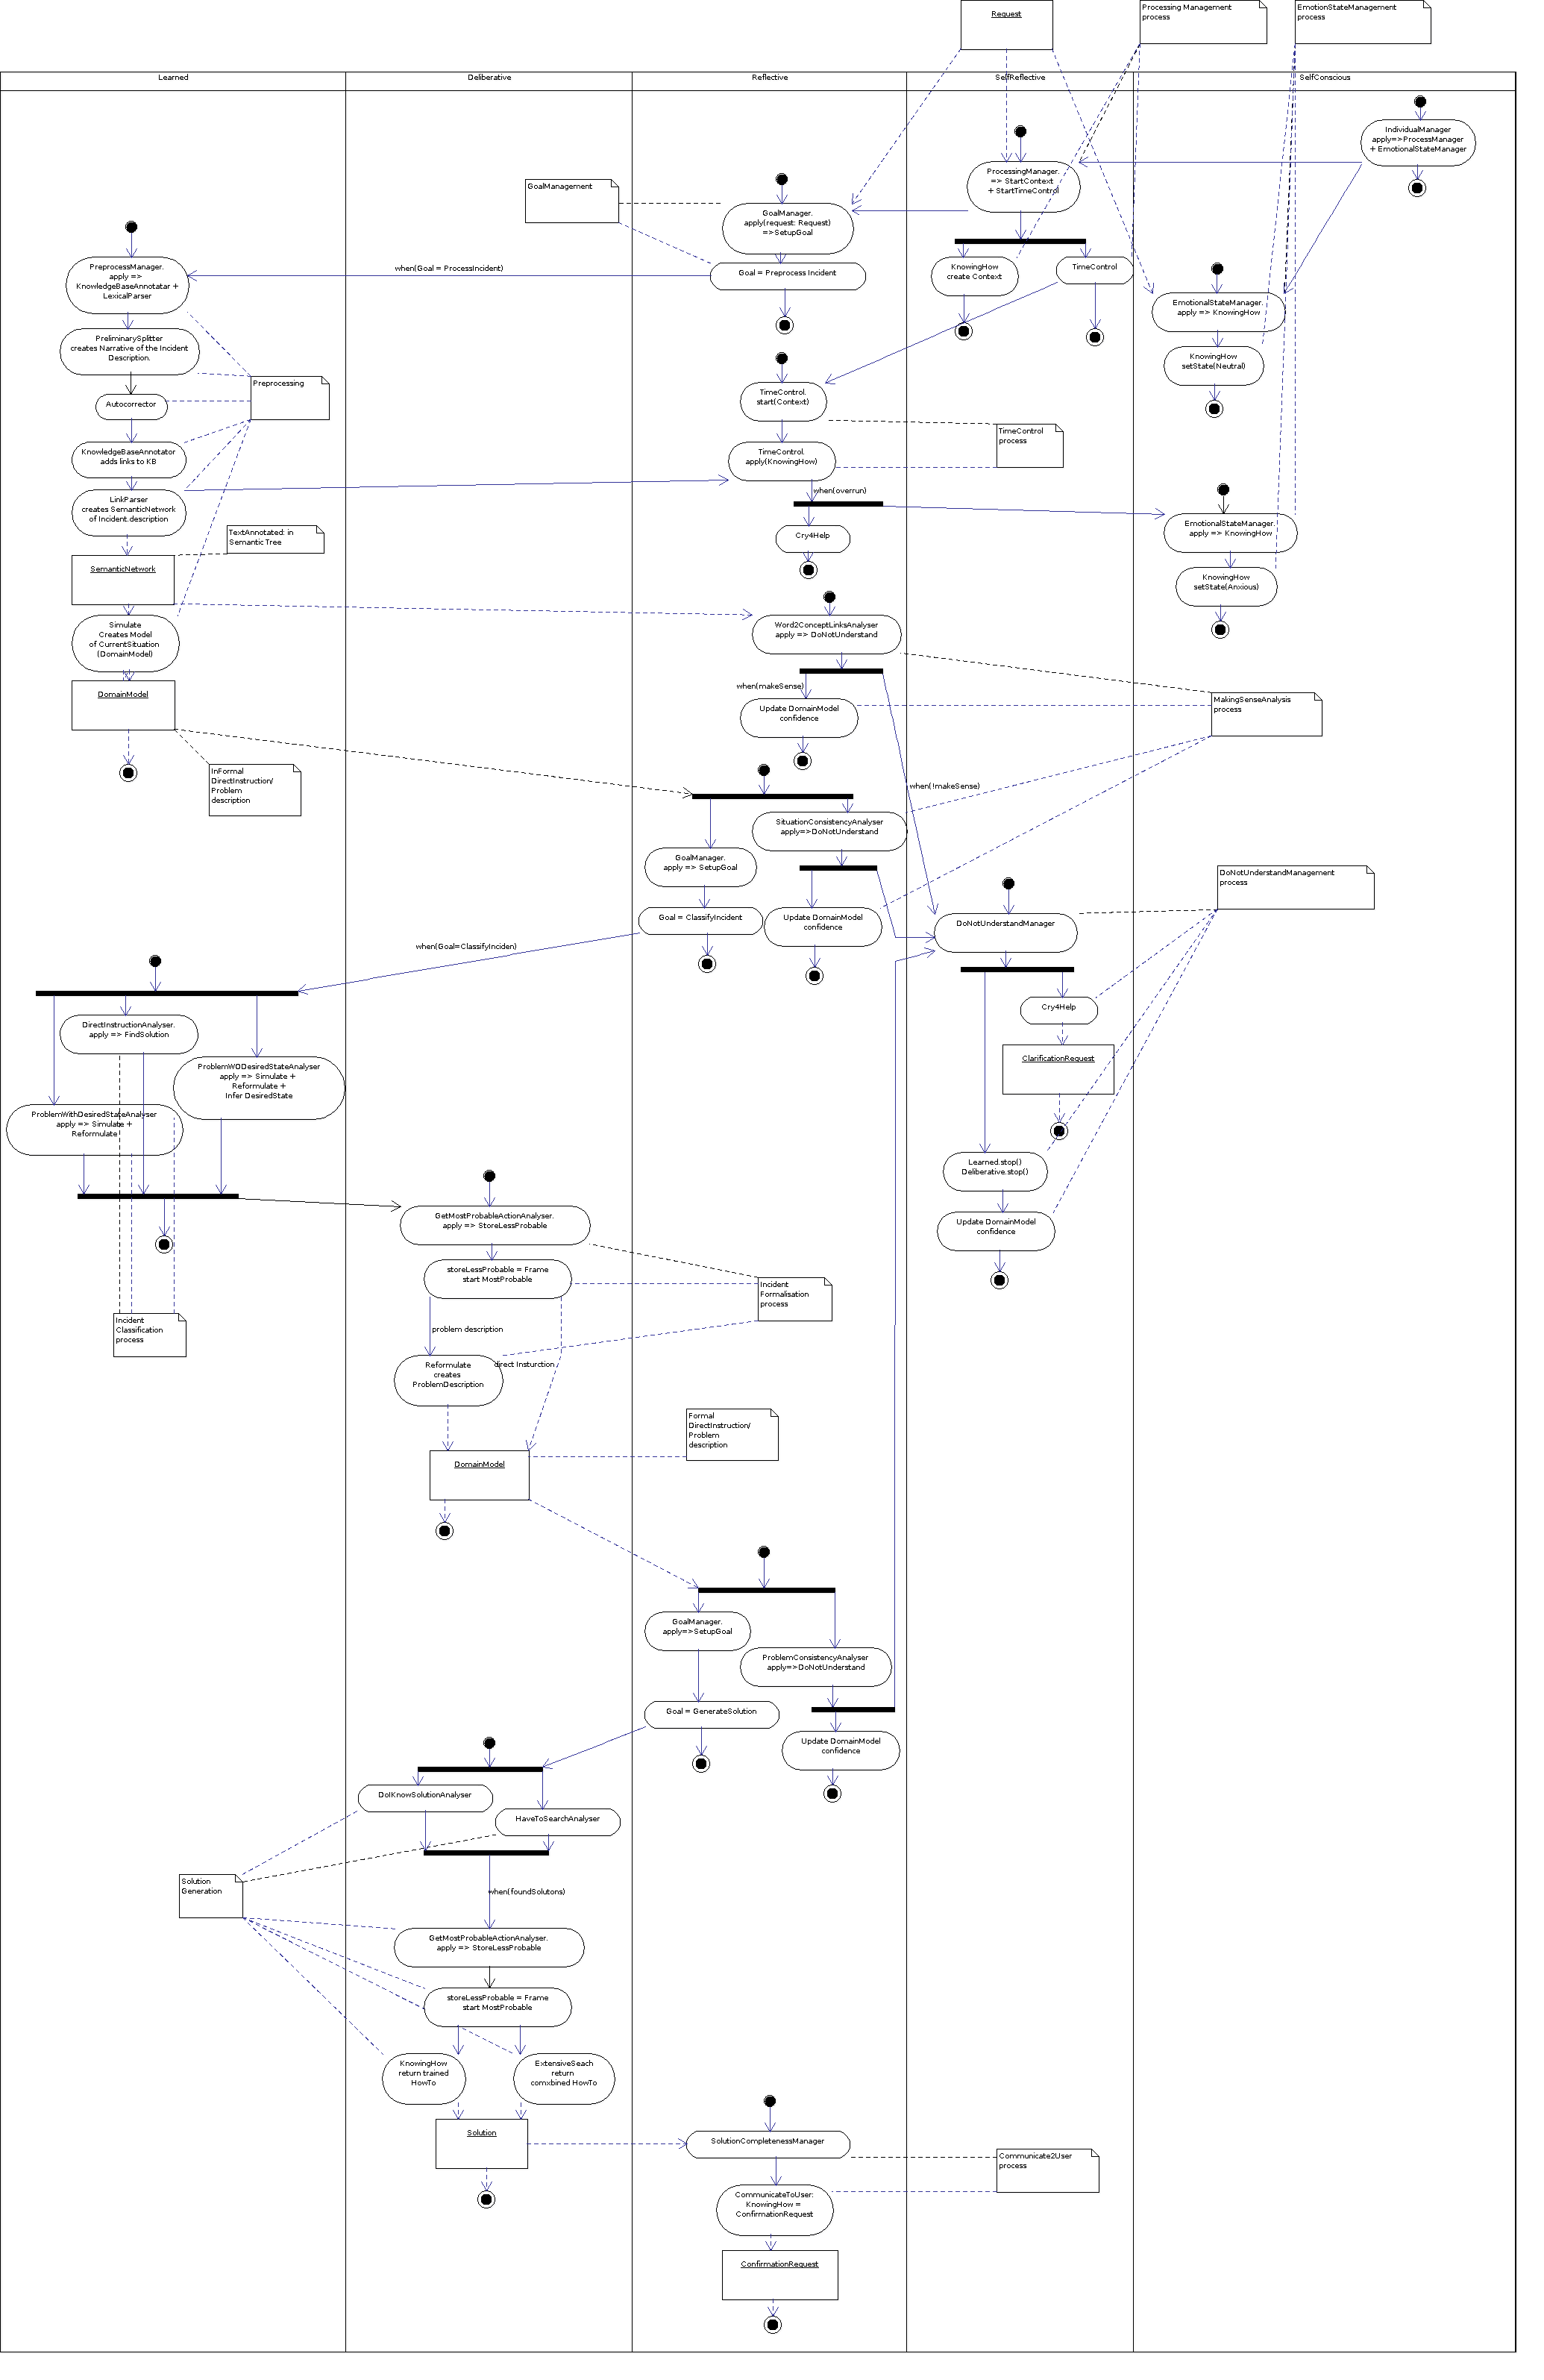
\includegraphics [scale=0.2] {LifecycleActivity}
  \caption{Диаграмма действий LifecycleActivity} 
  \label{img:LifecycleActivity}  
\end{figure}
\clearpage

\section{Выводы по главе 3}
В данной главе были рассмотрены:
\begin{itemize}
	\item архитектура системы по модели TU;
	\item модель данных TU Knowledge;
	\item реализация системы;
	\item состав прототипа;
	\item основной поток действий системы.
\end{itemize} \par
Кроме того, приведены алгоритмы и методы, использованные при создании системы; рассмотрены технологии, использованные при создании прототипа. Для удобства основные диаграммы выполнены с использованием универсального формата UML 2.0. В главе продемонстрированы основные потоки работы как для каждого компонента, так и для всех компонентов в целом. \par
По данной архитектуре была выполнена программная реализация с использованием функционального языка Scala. Основной платформой для эксплуатации системы был выбран Debian дистрибутив системы Linux, точнее, Ubuntu 12 (и выше). Связано это, прежде всего, с тем, что ряд компонентов был написан на С++ и использует библиотеки, доступные только на Linux.  \par
Система была протестирована на экспериментальных данных, которые представлены в Приложении \ref{AppendixE} и предоставлены \icl, о чем свидетельствует акт о внедрении (см. Приложение \ref{AppendixG}).


\clearpage